\chapter{پیاده‌سازی و توسعه مدل یادگیری ماشین}

در این فصل روش پیاده‌سازی مدل هوش مصنوعی را به تفصیل شرح خواهیم داد. ابتدا فرضیات و داده‌های ورودی و آماده‌ی تحلیل را مشخص کرده و نماد هر کدام را که تا انتهای این نوشته از آنها استفاده خواهیم کرد، مشخص می‌کنیم. در قسمت بعد مراحل پیش‌پردازش\LTRfootnote{Preprocess} را که روی این داده‌ها انجام می‌شود به ترتیب توضیح می‌دهیم و سپس ویژگی‌هایی که نیاز داریم از این داده‌های خام دربیاوریم را توضیح می‌دهیم و نحوه‌ی استخراج این ویژگی‌ها را نمایان می‌کنیم. در مرحله‌ی نهایی نحوه‌ی یادگیری مدل هوش مصنوعی و پیش‌بینی عمر باقی‌مانده‌ی دستگاه‌ها را بر اساس این ویژگی‌ها شرح می‌دهیم. در \cref{fig:analytics_structure}، قالب بسته‌ی هوش مصنوعی توسعه داده‌شده برای کارگزار اصلی را مشاهده می‌کنید که در این فصل به توضیح بخش‌های مختلف آن می‌پردازیم.

\begin{figure}[!h]
\centerline{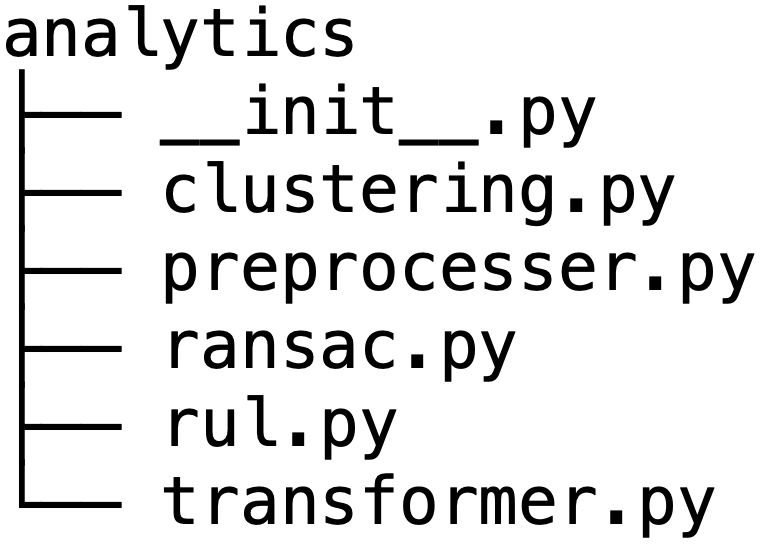
\includegraphics[width=0.4\textwidth]{analytics_structure.png}}
\caption{ساختار کلی بسته‌ی هوش مصنوعی}
\label{fig:analytics_structure}
\end{figure}



\section{توضیح مسئله}
با توجه به اینکه سیستم یادگیری ماشین بر اساس اطلاعات حسگرهای لرزش عمل می‌کند، برای داشتن کمترین خطا در عملیات پیش‌بینی باید فرضیاتی را پیش از طراحی و پیاده‌سازی سیستم در نظر داشته باشیم. اولاً نمونه‌های بدست‌آمده برای حسگرهای متفاوت بازه‌های زمانی مختلف را در بر می‌گیرند و همگن نیستند. ثانیاً این داده‌های دارای انحرافاتی در اندازه‌گیری بدلیل وجود گرانش یا خرابی حسگر هستند. ثالثاً وضعیت ابتدایی هر یک از گره‌هایی که می‌خواهیم اطلاعات لرزش آنها را جمع‌آوری و تحلیل کنیم یکی نیستند\cite{jung2017vibration}. با توجه به نکاتی که مطرح کردیم، پیاده‌کردن یک سیستم پیش‌پردازش و استخراج‌کننده‌ی ویژگی‌های مناسب، الزامی است. 

\begin{table}[h!]
  \begin{center}
    \caption{توضیحات نشانه‌گذاری داده‌ها}
    \label{table:notation_description}
    \begin{tabular}{|c|c|} % <-- Alignments: 1st column left and 2nd right with vertical lines in between
    	\hline
توضیحات & نشانه\\
    	\hline \hline
تعداد کل گره‌ها & $N$\\
    	\hline
 تعداد کل اندازه‌گیری‌ها & $M$\\
    	\hline
   تعداد کل نمونه‌های یک اندازه‌گیری & $K$\\
    	\hline
گره $n$ ام & $n$\\
 	\hline
اندازه‌گیری $m$ ام & $m$\\
 	\hline
نمونه‌ی $k$ ام یک اندازه‌گیری & $k$\\
 	\hline
بردار سه‌بعدی مربوط به اندازه‌گیری لرزش & $a_{nmk}$\\
 	\hline
بردار $k$بعدی مربوط به لرزش در محور $l \in \{x, y, z\}$  & $a^l_{nm}$\\
 	\hline
    \end{tabular}
  \end{center}
\end{table} 

\begin{table}[h!]
  \begin{center}
    \caption{برچسب‌های استفاده‌شده برای تعیین وضعیت دستگاه‌ها}
    \label{table:node_state_labels}
    \begin{tabular}{|c|c|} % <-- Alignments: 1st column left and 2nd right with vertical lines in between
    	\hline
توضیحات & برچسب\\
    	\hline \hline
دستگاه‌های نو که تازه تولید شده‌اند و آماده استفاده‌اند & $A$\\
    	\hline
دستگاه‌هایی که نو نیستند ولی هنوز مشغول کارکردن هستند & $B, C$\\
    	\hline
  دستگاه‌هایی خراب‌ شده‌اند یا در حال خرابی‌اند & $D$\\
    	\hline
    \end{tabular}
  \end{center}
\end{table}

در \cref{table:notation_description} توضیحات نشانه‌گذاری داده‌ی مربوط به این مسئله را می‌بینیم. همچنین در جهت مشخص کردن محدوده‌ی کاری این مسئله، از سه برچسب که در \cref{table:node_state_labels} مشخص شده‌اند، برای تعیین کردن وضعیت گره‌های موجود استفاده می‌کنیم.

\section{پیش‌پردازش}
این بخش وظیفه دارد قبل از انجام تحلیل داده، در ابتدا انحرافات و داده‌های پرت\LTRfootnote{Outlier Data} را از داده‌ی خام جدا کرده و داده‌ی قابل پردازش را به لایه‌ی بعد که لایه‌ی استخراج ویژگی‌ است تحویل دهد. در نهایت خروجی بخش پیش‌پردازنده، ویژگی‌هایی هستند که دستگاه یادگیری ماشین با تحلیل و بررسی آنها عملیات یادگیری و پیش‌بینی را انجام خواهد داد.

\subsection{از بین بردن انحرافات}
 حسگرهای کم‌هزینه \lr{MEMS} ،که داده‌های جمع‌آوری‌شده برای این پروژه توسط این نوع از حسگرها تأمین شده است، غالباً با گذشت زمان دچار انحرافاتی در اندازه‌گیری خواهند شد که منجر به اضافه یا کم شدن یک مقدار شتاب غیر صفر در اندازه‌گیری‌هایشان خواهد شد. از طرفی وجود گرانش، تاثیراتی روی اندازه‌گیری‌ها خواهد داشت و موجب ایجاد انحرافاتی رو به بالا یا پایین در این مقادیر خواهد شد\cite{jung2017vibration}. برای از بین بردن این مشکل همانطور که در \cref{eq:normalize} آورده شده است\cite{garcia2015data}، از هنجار‌کردن\LTRfootnote{Normalizing} داده با کم‌کردن میانگین مقادیر شتاب اندازه‌گیری شده در هر کدام از سه محور از مقادیر اندازه‌گیری‌شده استفاده کرده‌ایم. لازم به ذکر است همانطور که مشخص است، $\hat{a}^l_{nm}$ نماد ماتریس هنجار‌شده است.
\begin{equation}
\label{eq:normalize}
	\hat{a}^l_{nm}=a^l_{nm}-\sum_{k=1}^K \dfrac{a^l_{nmk}}{K}
\end{equation}


\subsection{از بین بردن داده‌های پرت}
در سیستم طراحی‌شده برای جمع‌آوری اطلاعات، ممکن است که تعدادی از حسگرها دچار مشکل شده باشند و داده‌ای که تحویل دروازه می‌دهند دقیق و در راستای داده‌های از قبل جمع‌آوری شده نباشد. به طور کلی، پایدار بودن میانگین شتاب دریافت‌شده از هر اندازه‌گیری، معیار خوبی برای تشخیص صحت و درستی اطلاعات جمع‌‌آوری شده است\cite{jung2017vibration}. به عبارتی دیگر، میانگین لرزش‌های اندازه گرفته‌شده نباید به طور ناگهانی بالا یا پایین روند و باید در همان حدود اندازه‌گیری‌های قبل باشند. برای جدا کردن این داده‌ها که اصطلاحا به آنها داده‌های پرت می‌گوییم، پیش از شروع یادگیری مدل، ابتدا میانگین شتاب جمع‌‌آوری ‌شده برای هر اندازه‌گیری موجود را در هر سه بعد حساب کرده و سپس با کمک یک الگوریتم خوشه‌بندی\LTRfootnote{Clustering}، این داده‌ها را جدا می‌کنیم.

برای انجام عملیات تشخیص داده‌های پرت، از الگوریتم خوشه‌بندی \lr{Mean Shift} استفاده کرده‌ایم که الگوریتمی بر اساس تخمین تراکم هسته\LTRfootnote{Kernel Density Estimate} می‌باشد. در \cref{fig:density_based_clustering}\cite{carreira2015review} نمونه‌ای از یک الگوریتم خوشه‌بندی تراکم‌محور آورده شده است. روند کار این الگوریتم بدین صورت است که به ازای ورودی به صورت نقاط و پارامتر ورودی پهنای باند\LTRfootnote{Bandwidth}، الگوریتم به طور مکرر هر نقطه داده را به نزدیکترین مرکز خوشه اختصاص می‌دهد و جهت نزدیکترین مرکز خوشه بر اساس جایی که اکثر نقاط نزدیک در آن قرار دارند تعیین می‌شود. در هر بار تکرار، هر نقطه داده به جایی که بیشترین نقاط در آن قرار دارد، نزدیکتر می‌شود، که در نهایت به مرکز خوشه منجر خواهد شد. هنگامی که الگوریتم متوقف می‌شود، هر نقطه به یک خوشه اختصاص داده می‌شود. همانطور که گفته‌شد، این الگوریتم بغیر از پهنای باند به پارامتر دیگری نیاز ندارد. این امر سبب می‌شود که مواردی همانند تعداد و مراکز هر خوشه، توسط خود الگوریتم مشخص شوند\cite{carreira2015review}.

\begin{figure}[!h]
\centerline{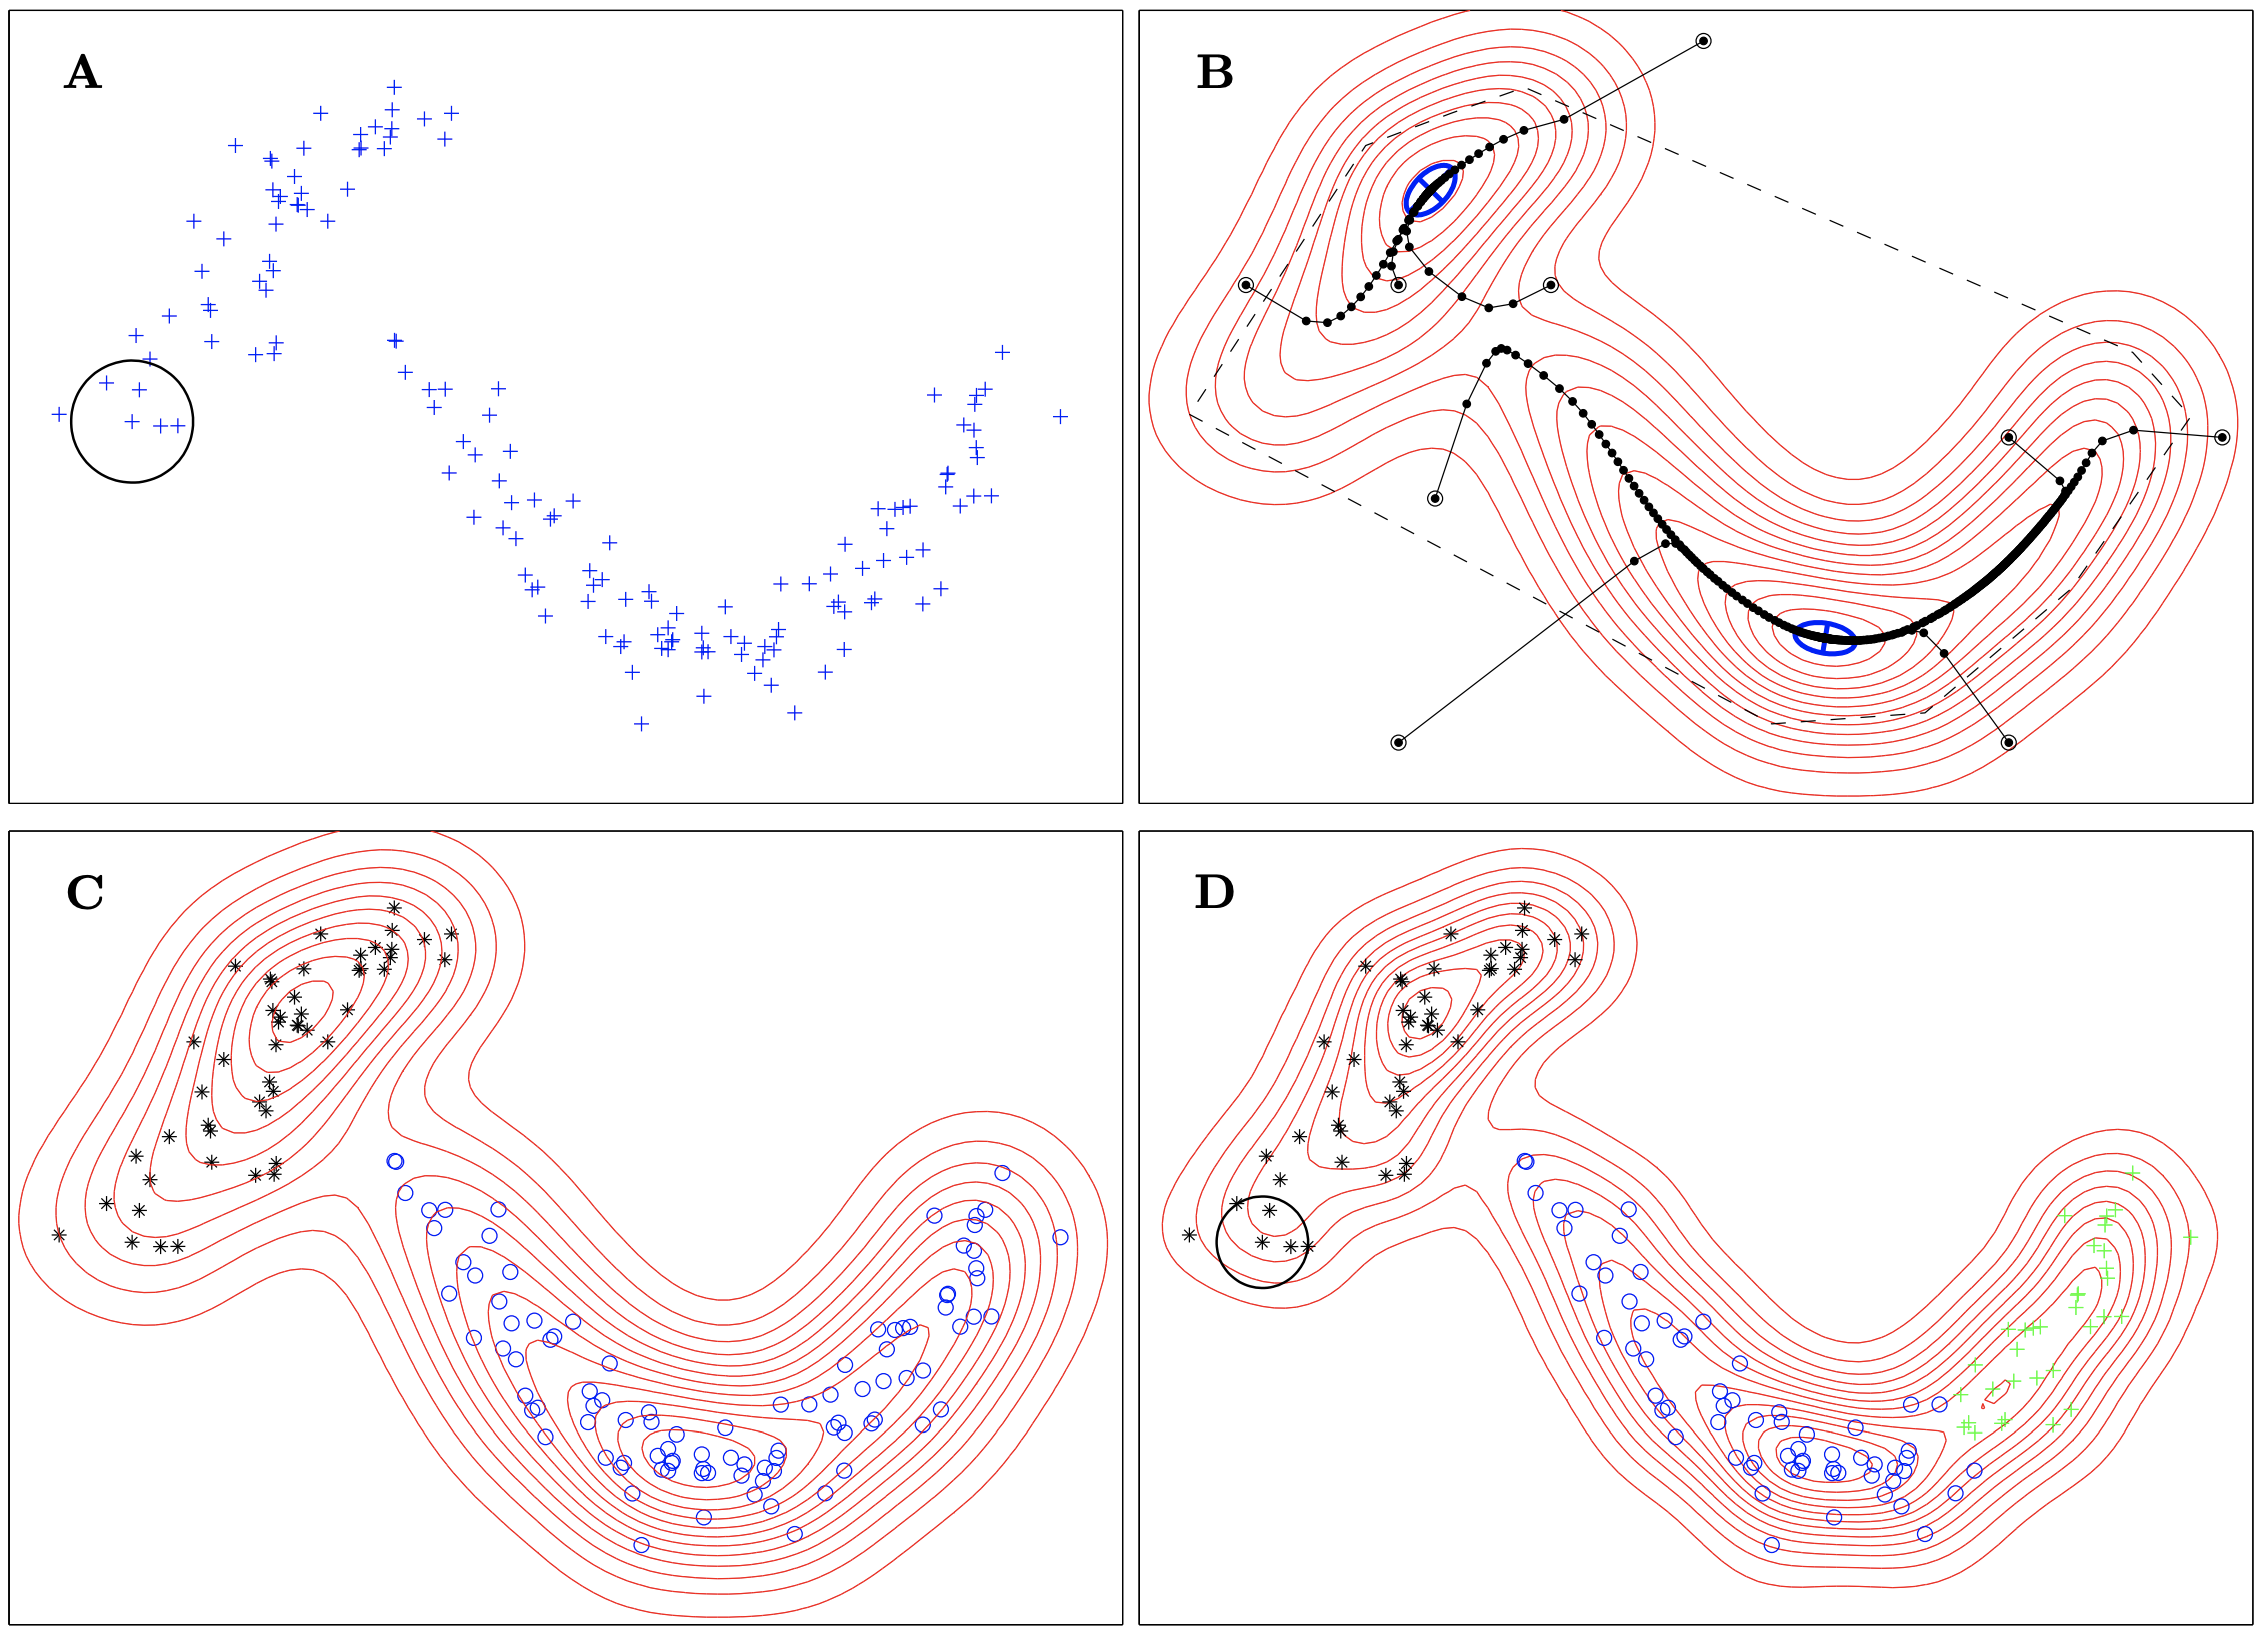
\includegraphics[width=\textwidth]{density_based_clustering.png}}
\caption{روند خوشه‌بندی یک الگوریتم تراکم‌محور\cite{carreira2015review}}
\label{fig:density_based_clustering}
\end{figure}



\subsection{استخراج ویژگی‌ها}
تا اینجای کار، اثرهای انحرافات ممکن را از بین بردیم و داده‌های پرت را از میان کل داده‌ها جدا کردیم. از آنجا که داده‌ی خام لرزش گره‌های موجود در شبکه‌ی اشیاء، در دامنه‌ی زمانی\LTRfootnote{Time Domain} بوده و حالت شروع به کار و وضعیت فعلی هر کدام از آنها در حال حاضر با همدیگر متفاوت است، نیازمند آنیم که از این داده‌های خام، ویژگی‌هایی مناسب را جهت انجام تحلیل و یادگیری ماشین، استخراج کنیم؛ برای این منظور بردن داده‌های موجود در دامنه زمانی به دامنه‌ی فرکانسی با کمک تبدیل فوریه\LTRfootnote{Fourier Transform}، شروع خوبی است.


\section{نحوه‌ی یادگیری مدل}

\subsection{محاسبه‌ی مشابهت بین وضعیت دستگاه‌ها}

\subsection{پیاده‌کردن مدل}


\section{جمع‌بندی و نتیجه‌گیری}
این بخش به طور دقیق روند یادگیری ماشین از اطلاعات لرزش گره‌ها را نشان داد. مشخص شد که داده‌های جمع‌آوری شده ابتدا به کمک پیش‌پردازنده که شامل هنجارکننده، تشخیص‌دهنده‌ی داده‌ی پرت و استخراج‌کننده‌ی ویژگی‌های آماده پردازش است، پالایش شده و سپس تحویل واحد یادگیری ماشین می‌شود. در این مرحله این واحد با انتخاب کردن ۲۰ تا از بیشترین مقادیر موزون ویژگی \lr{PSD} برای هر اندازه‌گیری، اقدام به محاسبه‌ی میزان شباهت این اندازه‌گیری‌ها به اندازه‌گیری‌های یک دستگاه سالم می‌کند و بنا به میزان شباهت یا تفاوت با آن، پیش‌بینی مربوط به طول عمر باقی‌مانده‌ی گره را خروجی خواهد داد.